%%%%%%%%%%%%%%%%%%%%%%%%%%%%%%%%%%%%%%%%%%%%%%%%%%%%%%%%%%%%%%%%%%%%%%%%%%%%%%%
\section{Borealis basics}\label{sec:basics}
%%%%%%%%%%%%%%%%%%%%%%%%%%%%%%%%%%%%%%%%%%%%%%%%%%%%%%%%%%%%%%%%%%%%%%%%%%%%%%%

This work is based on Borealis bounded model checker~\cite{Borealis}, which used for C programming language. A large-scale overview of Borealis is shown in figure~\ref{fig:borealis-scheme}.

\begin{figure}[tbh]
\centering
\caption{High-level scheme of Borealis bounded model checker}
\label{fig:borealis-scheme}
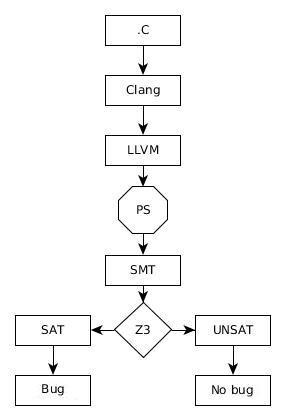
\includegraphics[keepaspectratio, width=\linewidth, height=8cm]{BorSch}
\end{figure}

Borealis based on LLVM \cite{LLVM} framework, it works by converting a program representation to SMT formulae, which is then checked for possible satisfiability. Borealis uses its own program representation named Predicate State~(PS). PS for given LLVM instruction corresponds to SMT formulae, which describes all possible program states in this instruction. PS for a given LLVM~IR instruction corresponds to an SMT formula, which describes all possible program states at this instruction. A simplified description of PS format is shown in figure~\ref{fig:predicate-state}.

\renewcommand{\litleft}{\bfshape}
\renewcommand{\litright}{}

\begin{figure*}[p]

\caption{Predicate state format}
\label{fig:predicate-state}

\begin{grammar}

<PredicateState> ::= "PredicateStateChain" head:<PredicateState> tail:<PredicateState>
\alt "PredicateStateChoice" choices:<ListOfPredicateStates>
\alt "BasicPredicateState" data:<ListOfPredicates>

<Predicate> ::= "AllocaPredicate" lhv:<Term> numElems:<Term> origNumElems:<Term>
\alt "DefaultSwitchCasePredicate" cond:<Term> cases:<ListOfTerms>
\alt "EqualityPredicate" lhv:<Term> rhv:<Term>
\alt "GlobalsPredicate" globals:<ListOfTerms>
\alt "InequalityPredicate" lhv:<Term> rhv:<Term>
\alt "MallocPredicate" lhv:<Term> numElems:<Term> origNumElems:<Term>
\alt "SeqDataPredicate" base:<Term> data:<ListOfTerms>
\alt "SeqDataZeroPredicate" base:<Term> size:\textit{UInt32}
\alt "StorePredicate" ptr:<Term> value:<Term>
\alt "WriteBoundPredicate" ptr:<Term> boundValue:<Term>
\alt "WritePropertyPredicate" propName:<Term> ptr:<Term> propValue:<Term>

<Term> ::= "ArgumentTerm" idx:\textit{UInt32} kind:<ArgumentKind>
\alt "ArgumentCountTerm"
\alt "AxiomTerm" term:<Term> axiom:<Term>
\alt "BinaryTerm" op:<BinaryOp> lhv:<Term> rhv:<Term>
\alt "BoundTerm" term:<Term>
\alt "CastTerm" term:<Term> signExtend:\textit{Bool}
\alt "CmpTerm" op:<CmpOp> lhv:<Term> rhv:<Term>
\alt "ConstTerm"
\alt "FreeVarTerm"
\alt "GepTerm" base:<Term> shifts:<ListOfTerms> triviallyInbounds:\textit{Bool}
\alt "LoadTerm" ptr:<Term>
\alt "ReadPropertyTerm" propName:<Term> ptr:<Term>
\alt "ReturnPtrTerm" funcName:\textit{String}
\alt "ReturnValueTerm" funcName:\textit{String}
\alt "SignTerm" value:<Term>
\alt "TernaryTerm" cond:<Term> tru:<Term> fls:<Term>
\alt "UnaryTerm" op:<UnaryOp> value:<Term>
\alt "ValueTerm" global:\textit{Bool}
\alt "VarArgumentTerm" index:\textit{UInt32}
\alt ...

<ListOfPredicateStates> ::= <PredicateState> <ListOfPredicateStates> | <empty>

<ListOfPredicates> ::= <Predicate> <ListOfPredicates> | <empty>

<ListOfTerms> ::= <Term> <ListOfTerms> | <empty>

<ArgumentKind> ::= "ANY" | "STRING"

<CmpOp> ::= "EQ" | "NEQ" | "GT" | ...

<BinaryOp> ::=  "ADD" | "SUB" | "MUL" | ...

<UnaryOp> ::= "NEG" | "NOT" | "BINARY_NOT"

\end{grammar}
\end{figure*}


Functions approximations can be hand-crafted by the user in the form of source code or external annotations or external tools for component description. Also approximations can be extracted from source code using Craig interpolation or dynamic analyses. In this work we represented yet another approach to function approximation based on extraction from source code.